% Options for packages loaded elsewhere
\PassOptionsToPackage{unicode}{hyperref}
\PassOptionsToPackage{hyphens}{url}
%
\documentclass[
]{article}
\usepackage{amsmath,amssymb}
\usepackage{lmodern}
\usepackage{iftex}
\ifPDFTeX
  \usepackage[T1]{fontenc}
  \usepackage[utf8]{inputenc}
  \usepackage{textcomp} % provide euro and other symbols
\else % if luatex or xetex
  \usepackage{unicode-math}
  \defaultfontfeatures{Scale=MatchLowercase}
  \defaultfontfeatures[\rmfamily]{Ligatures=TeX,Scale=1}
\fi
% Use upquote if available, for straight quotes in verbatim environments
\IfFileExists{upquote.sty}{\usepackage{upquote}}{}
\IfFileExists{microtype.sty}{% use microtype if available
  \usepackage[]{microtype}
  \UseMicrotypeSet[protrusion]{basicmath} % disable protrusion for tt fonts
}{}
\makeatletter
\@ifundefined{KOMAClassName}{% if non-KOMA class
  \IfFileExists{parskip.sty}{%
    \usepackage{parskip}
  }{% else
    \setlength{\parindent}{0pt}
    \setlength{\parskip}{6pt plus 2pt minus 1pt}}
}{% if KOMA class
  \KOMAoptions{parskip=half}}
\makeatother
\usepackage{xcolor}
\usepackage[margin=1in]{geometry}
\usepackage{color}
\usepackage{fancyvrb}
\newcommand{\VerbBar}{|}
\newcommand{\VERB}{\Verb[commandchars=\\\{\}]}
\DefineVerbatimEnvironment{Highlighting}{Verbatim}{commandchars=\\\{\}}
% Add ',fontsize=\small' for more characters per line
\usepackage{framed}
\definecolor{shadecolor}{RGB}{248,248,248}
\newenvironment{Shaded}{\begin{snugshade}}{\end{snugshade}}
\newcommand{\AlertTok}[1]{\textcolor[rgb]{0.94,0.16,0.16}{#1}}
\newcommand{\AnnotationTok}[1]{\textcolor[rgb]{0.56,0.35,0.01}{\textbf{\textit{#1}}}}
\newcommand{\AttributeTok}[1]{\textcolor[rgb]{0.77,0.63,0.00}{#1}}
\newcommand{\BaseNTok}[1]{\textcolor[rgb]{0.00,0.00,0.81}{#1}}
\newcommand{\BuiltInTok}[1]{#1}
\newcommand{\CharTok}[1]{\textcolor[rgb]{0.31,0.60,0.02}{#1}}
\newcommand{\CommentTok}[1]{\textcolor[rgb]{0.56,0.35,0.01}{\textit{#1}}}
\newcommand{\CommentVarTok}[1]{\textcolor[rgb]{0.56,0.35,0.01}{\textbf{\textit{#1}}}}
\newcommand{\ConstantTok}[1]{\textcolor[rgb]{0.00,0.00,0.00}{#1}}
\newcommand{\ControlFlowTok}[1]{\textcolor[rgb]{0.13,0.29,0.53}{\textbf{#1}}}
\newcommand{\DataTypeTok}[1]{\textcolor[rgb]{0.13,0.29,0.53}{#1}}
\newcommand{\DecValTok}[1]{\textcolor[rgb]{0.00,0.00,0.81}{#1}}
\newcommand{\DocumentationTok}[1]{\textcolor[rgb]{0.56,0.35,0.01}{\textbf{\textit{#1}}}}
\newcommand{\ErrorTok}[1]{\textcolor[rgb]{0.64,0.00,0.00}{\textbf{#1}}}
\newcommand{\ExtensionTok}[1]{#1}
\newcommand{\FloatTok}[1]{\textcolor[rgb]{0.00,0.00,0.81}{#1}}
\newcommand{\FunctionTok}[1]{\textcolor[rgb]{0.00,0.00,0.00}{#1}}
\newcommand{\ImportTok}[1]{#1}
\newcommand{\InformationTok}[1]{\textcolor[rgb]{0.56,0.35,0.01}{\textbf{\textit{#1}}}}
\newcommand{\KeywordTok}[1]{\textcolor[rgb]{0.13,0.29,0.53}{\textbf{#1}}}
\newcommand{\NormalTok}[1]{#1}
\newcommand{\OperatorTok}[1]{\textcolor[rgb]{0.81,0.36,0.00}{\textbf{#1}}}
\newcommand{\OtherTok}[1]{\textcolor[rgb]{0.56,0.35,0.01}{#1}}
\newcommand{\PreprocessorTok}[1]{\textcolor[rgb]{0.56,0.35,0.01}{\textit{#1}}}
\newcommand{\RegionMarkerTok}[1]{#1}
\newcommand{\SpecialCharTok}[1]{\textcolor[rgb]{0.00,0.00,0.00}{#1}}
\newcommand{\SpecialStringTok}[1]{\textcolor[rgb]{0.31,0.60,0.02}{#1}}
\newcommand{\StringTok}[1]{\textcolor[rgb]{0.31,0.60,0.02}{#1}}
\newcommand{\VariableTok}[1]{\textcolor[rgb]{0.00,0.00,0.00}{#1}}
\newcommand{\VerbatimStringTok}[1]{\textcolor[rgb]{0.31,0.60,0.02}{#1}}
\newcommand{\WarningTok}[1]{\textcolor[rgb]{0.56,0.35,0.01}{\textbf{\textit{#1}}}}
\usepackage{longtable,booktabs,array}
\usepackage{calc} % for calculating minipage widths
% Correct order of tables after \paragraph or \subparagraph
\usepackage{etoolbox}
\makeatletter
\patchcmd\longtable{\par}{\if@noskipsec\mbox{}\fi\par}{}{}
\makeatother
% Allow footnotes in longtable head/foot
\IfFileExists{footnotehyper.sty}{\usepackage{footnotehyper}}{\usepackage{footnote}}
\makesavenoteenv{longtable}
\usepackage{graphicx}
\makeatletter
\def\maxwidth{\ifdim\Gin@nat@width>\linewidth\linewidth\else\Gin@nat@width\fi}
\def\maxheight{\ifdim\Gin@nat@height>\textheight\textheight\else\Gin@nat@height\fi}
\makeatother
% Scale images if necessary, so that they will not overflow the page
% margins by default, and it is still possible to overwrite the defaults
% using explicit options in \includegraphics[width, height, ...]{}
\setkeys{Gin}{width=\maxwidth,height=\maxheight,keepaspectratio}
% Set default figure placement to htbp
\makeatletter
\def\fps@figure{htbp}
\makeatother
\setlength{\emergencystretch}{3em} % prevent overfull lines
\providecommand{\tightlist}{%
  \setlength{\itemsep}{0pt}\setlength{\parskip}{0pt}}
\setcounter{secnumdepth}{-\maxdimen} % remove section numbering
\ifLuaTeX
  \usepackage{selnolig}  % disable illegal ligatures
\fi
\IfFileExists{bookmark.sty}{\usepackage{bookmark}}{\usepackage{hyperref}}
\IfFileExists{xurl.sty}{\usepackage{xurl}}{} % add URL line breaks if available
\urlstyle{same} % disable monospaced font for URLs
\hypersetup{
  pdftitle={2nd homework assignment},
  hidelinks,
  pdfcreator={LaTeX via pandoc}}

\title{2nd homework assignment}
\author{}
\date{\vspace{-2.5em}}

\begin{document}
\maketitle

\hypertarget{task-1---maximum-likelihood-method-6-points}{%
\subsection{Task 1 - Maximum likelihood method (6
points)}\label{task-1---maximum-likelihood-method-6-points}}

Firstly, generate your own \texttt{data1} containing 100 observations.
Do not forget to change set.seed() of PRNG with your UČO:

\begin{Shaded}
\begin{Highlighting}[]
\NormalTok{uco }\OtherTok{\textless{}{-}} \DecValTok{492875}  \CommentTok{\# insert your UCO}
\FunctionTok{set.seed}\NormalTok{(uco)}
\NormalTok{data1 }\OtherTok{\textless{}{-}} \FunctionTok{round}\NormalTok{(}\FunctionTok{rgamma}\NormalTok{(}\DecValTok{100}\NormalTok{, }\DecValTok{1}\NormalTok{, }\DecValTok{1}\SpecialCharTok{/}\DecValTok{5}\NormalTok{), }\DecValTok{2}\NormalTok{)}
\NormalTok{data1 }\OtherTok{\textless{}{-}}\NormalTok{ data1[data1 }\SpecialCharTok{!=} \DecValTok{0}\NormalTok{]}
\end{Highlighting}
\end{Shaded}

If there is a 0 present in your data. Ignore such observation. Consider
that the data represent waiting time in \(minutes\) in a queue at the
study department of 100 randomly selected students.

\begin{enumerate}
\def\labelenumi{\alph{enumi})}
\tightlist
\item
  Fit exponential distribution with parameter \(\lambda\) to your data
  (use the same parametrization as in the lecture). Use numerical
  maximization of the corresponding log-likelihood function to find the
  maximum likelihood estimate of \(\lambda\).
\end{enumerate}

\begin{longtable}[]{@{}l@{}}
\toprule()
\(\widehat{\lambda}\) \\
\midrule()
\endhead
\texttt{0.170711} \\
\bottomrule()
\end{longtable}

\begin{enumerate}
\def\labelenumi{\alph{enumi})}
\setcounter{enumi}{1}
\tightlist
\item
  Fit lognormal distribution with parameters \(\mu\) and \(\sigma\) with
  probability density function
  \[ f(x)=\begin{cases} \frac{1}{x \sigma \sqrt{2 \pi}} \textrm{e}^{-\frac{(\log x - \mu)^2}{2\sigma^2
  }}, &\ x \geq 0, \\
  0, &\ \mbox{otherwise}
  \\ \end{cases}
  \] on your data (see \verb'?dlnorm' in \verb'R' for details). Use
  numerical maximization of the corresponding log-likelihood function to
  find the maximum likelihood estimates of \(\mu\) and \(\sigma\).
\end{enumerate}

\begin{longtable}[]{@{}ll@{}}
\toprule()
\(\widehat{\mu}\) & \(\widehat{\sigma}\) \\
\midrule()
\endhead
\texttt{1.111128} & \texttt{1.411239} \\
\bottomrule()
\end{longtable}

\begin{enumerate}
\def\labelenumi{\alph{enumi})}
\setcounter{enumi}{2}
\tightlist
\item
  Plot histogram of your data together with both estimated densities.
\end{enumerate}

\includegraphics[width=0.7\linewidth]{homework_assignment_2_files/figure-latex/unnamed-chunk-2-1}

\begin{enumerate}
\def\labelenumi{\alph{enumi})}
\setcounter{enumi}{3}
\tightlist
\item
  Which of the two models would you choose? Why? Support your conclusion
  with a numerical characteristic.
\end{enumerate}

\begin{longtable}[]{@{}
  >{\raggedright\arraybackslash}p{(\columnwidth - 2\tabcolsep) * \real{0.2222}}
  >{\raggedright\arraybackslash}p{(\columnwidth - 2\tabcolsep) * \real{0.7778}}@{}}
\toprule()
\begin{minipage}[b]{\linewidth}\raggedright
Chosen model
\end{minipage} & \begin{minipage}[b]{\linewidth}\raggedright
Explanation
\end{minipage} \\
\midrule()
\endhead
\texttt{Exponential} & The dataset seems to be closer to exponential
distribution rather than the lognormal. Using qqnorm, the lower tail
part of the dataset seems to follow the exponential distribution much
better than the lognormal distribution. \\
\bottomrule()
\end{longtable}

\begin{enumerate}
\def\labelenumi{\alph{enumi})}
\setcounter{enumi}{4}
\tightlist
\item
  Based on both estimated models, what is the probability that you will
  wait in a queue for more than 5 minutes?
\end{enumerate}

\begin{longtable}[]{@{}
  >{\raggedright\arraybackslash}p{(\columnwidth - 2\tabcolsep) * \real{0.5833}}
  >{\raggedright\arraybackslash}p{(\columnwidth - 2\tabcolsep) * \real{0.4167}}@{}}
\toprule()
\begin{minipage}[b]{\linewidth}\raggedright
Estimated probability for exponential model
\end{minipage} & \begin{minipage}[b]{\linewidth}\raggedright
Estimated probability for lognormal model
\end{minipage} \\
\midrule()
\endhead
0.4258981 & 0.3620063 \\
\bottomrule()
\end{longtable}

\hypertarget{task-2---statistics-i-2-points}{%
\subsection{Task 2 - Statistics I (2
points)}\label{task-2---statistics-i-2-points}}

Work with the same data as in the previous task. Use the knowledge that
the data represent waiting time in \textbf{minutes} between individual
events. Using your result from the previous task, estimate the number of
students coming to the study department in \textbf{one hour}. Construct
a corresponding confidence interval.

\begin{longtable}[]{@{}lll@{}}
\toprule()
Estimated number of students & Confidence interval & \\
\midrule()
\endhead
\texttt{10.24266} & \texttt{{[}4.663266,\ 7.051334{]}} & \\
\bottomrule()
\end{longtable}

\hypertarget{task-3---normality-checking-3-points}{%
\subsection{Task 3 - Normality checking (3
points)}\label{task-3---normality-checking-3-points}}

Again, start with obtaining your data as a random sample from
\texttt{data1}.

\begin{Shaded}
\begin{Highlighting}[]
\NormalTok{uco }\OtherTok{\textless{}{-}} \DecValTok{492875}  \CommentTok{\# insert your UCO}
\FunctionTok{set.seed}\NormalTok{(uco)}
\NormalTok{data2 }\OtherTok{\textless{}{-}} \FunctionTok{sample}\NormalTok{(data1, }\DecValTok{80}\NormalTok{)}
\end{Highlighting}
\end{Shaded}

The aim of this task is to decide whether your data might come from a
normal distribution. You can use any methods of your choosing, but for
the purposes of this task, present only your final decision supported by
one graph and the results of one statistical test.

\begin{longtable}[]{@{}l@{}}
\toprule()
Do your data look normal? \\
\midrule()
\endhead
\texttt{no} \\
\bottomrule()
\end{longtable}

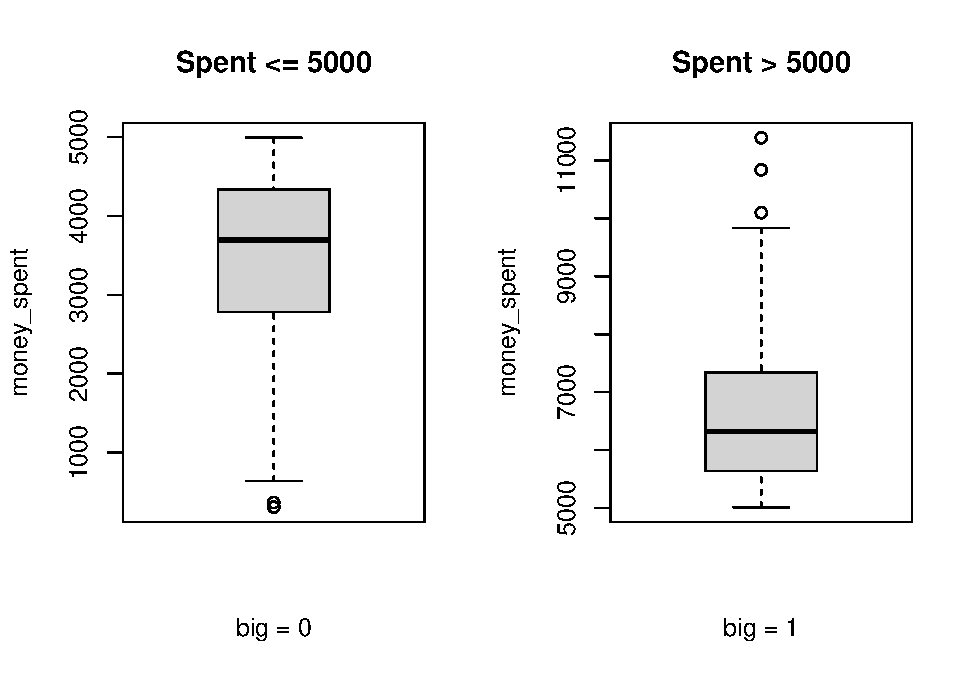
\includegraphics[width=0.7\linewidth]{homework_assignment_2_files/figure-latex/unnamed-chunk-4-1}

Support your claim with ONE suitable plot and a result of ONE
statistical test confirming it.

\begin{longtable}[]{@{}ll@{}}
\toprule()
Name of the test & p-value \\
\midrule()
\endhead
\texttt{Shapiro-Wilk\ Test} & \texttt{8.439703e-09} \\
\bottomrule()
\end{longtable}

\hypertarget{task-4---statistics-ii-4-points}{%
\subsection{Task 4 - Statistics II (4
points)}\label{task-4---statistics-ii-4-points}}

In assignment 1, we worked with the \textbf{customer\_behaviour2}
dataset and created a new variable called \texttt{big} with values 1
(\texttt{big\ spender}, if the person spent more money than 5000 USD),
and 0 (\texttt{low\ spender}, if he spent less or equal). The question
is whether the big spenders are rather older people and the low spenders
tend to be younger?

\begin{enumerate}
\def\labelenumi{\alph{enumi})}
\tightlist
\item
  Use a suitable model and formulate null and alternative hypotheses and
  choose an appropriate test.
\end{enumerate}

\begin{longtable}[]{@{}
  >{\raggedright\arraybackslash}p{(\columnwidth - 2\tabcolsep) * \real{0.1944}}
  >{\raggedright\arraybackslash}p{(\columnwidth - 2\tabcolsep) * \real{0.8056}}@{}}
\toprule()
\begin{minipage}[b]{\linewidth}\raggedright
Name of the test you used
\end{minipage} & \begin{minipage}[b]{\linewidth}\raggedright
Explanation of your choice
\end{minipage} \\
\midrule()
\endhead
\texttt{Two-sample\ t-test} &
\texttt{We\ are\ comparing\ the\ ages\ of\ two\ different\ groups\ of\ individuals\ (big\ spenders\ and\ low\ spenders)\ to\ test\ whether\ there\ is\ a\ statistically\ significant\ difference\ in\ their\ age\ distributions.} \\
\bottomrule()
\end{longtable}

Perform the test.

\begin{Shaded}
\begin{Highlighting}[]
\CommentTok{\#load and process data}
\FunctionTok{load}\NormalTok{(}\StringTok{"customer\_behaviour2.RData"}\NormalTok{)}
\NormalTok{data}\SpecialCharTok{$}\NormalTok{big }\OtherTok{=} \FunctionTok{as.numeric}\NormalTok{(data}\SpecialCharTok{$}\NormalTok{money\_spent }\SpecialCharTok{\textgreater{}} \DecValTok{5000}\NormalTok{)}
\NormalTok{big\_spenders }\OtherTok{=}\NormalTok{ data[data}\SpecialCharTok{$}\NormalTok{big }\SpecialCharTok{==} \DecValTok{1}\NormalTok{,]}\SpecialCharTok{$}\NormalTok{age}
\NormalTok{small\_spenders }\OtherTok{=}\NormalTok{ data[data}\SpecialCharTok{$}\NormalTok{big }\SpecialCharTok{==} \DecValTok{0}\NormalTok{,]}\SpecialCharTok{$}\NormalTok{age}

\CommentTok{\#two{-}tailed t{-}test to test if there is indeed a difference}
\CommentTok{\#H0 {-} There is not a significant difference between big and small spender}
\CommentTok{\#HA {-} There is a significant difference}
\NormalTok{result }\OtherTok{=} \FunctionTok{t.test}\NormalTok{(big\_spenders, small\_spenders)}
\FunctionTok{ifelse}\NormalTok{(result}\SpecialCharTok{$}\NormalTok{p.value }\SpecialCharTok{\textless{}}\FloatTok{0.05}\NormalTok{, }\StringTok{"H0 rejected"}\NormalTok{, }\StringTok{"Failed to reject H0"}\NormalTok{)}
\end{Highlighting}
\end{Shaded}

\begin{verbatim}
## [1] "H0 rejected"
\end{verbatim}

\begin{Shaded}
\begin{Highlighting}[]
\CommentTok{\#H0 rejected {-}\textgreater{} statistically significant evidence that}
    \CommentTok{\#there is a difference in age in both groups}
\CommentTok{\#failed to reject H0 {-}\textgreater{} not enough statistically significant}
    \CommentTok{\#evidence to tell if there is a difference in age of both groups}

\CommentTok{\#test the direction of the difference}
\FunctionTok{ifelse}\NormalTok{(}\FunctionTok{mean}\NormalTok{(big\_spenders) }\SpecialCharTok{\textless{}} \FunctionTok{mean}\NormalTok{(small\_spenders),}
       \StringTok{"Big spenders are statistically younger"}\NormalTok{,}
       \StringTok{"Big spenders are statistically older"}\NormalTok{)}
\end{Highlighting}
\end{Shaded}

\begin{verbatim}
## [1] "Big spenders are statistically younger"
\end{verbatim}

What is you conclusion?

\begin{longtable}[]{@{}
  >{\raggedright\arraybackslash}p{(\columnwidth - 4\tabcolsep) * \real{0.2055}}
  >{\raggedright\arraybackslash}p{(\columnwidth - 4\tabcolsep) * \real{0.2055}}
  >{\raggedright\arraybackslash}p{(\columnwidth - 4\tabcolsep) * \real{0.5890}}@{}}
\toprule()
\begin{minipage}[b]{\linewidth}\raggedright
p-value of the test
\end{minipage} & \begin{minipage}[b]{\linewidth}\raggedright
Formal conclusion
\end{minipage} & \begin{minipage}[b]{\linewidth}\raggedright
Conclusion with your own words
\end{minipage} \\
\midrule()
\endhead
\texttt{2.2e-16} & Reject H0 &
\texttt{Based\ on\ the\ two-tailed\ t-test\ result,\ I\ can\ reject\ the\ null\ hypothesis.\ This\ means\ that\ there\ is\ a\ statistically\ significant\ difference\ in\ the\ age\ of\ both\ groups.\ By\ comparing\ their\ means,\ I\ can\ determine\ the\ direction\ of\ this\ difference.\ This\ tells\ me\ that\ bigger\ spenders\ tend\ to\ be\ younger\ rather\ than\ older.} \\
\bottomrule()
\end{longtable}

\begin{enumerate}
\def\labelenumi{\alph{enumi})}
\setcounter{enumi}{1}
\tightlist
\item
  Construct the corresponding confidence interval and use it for testing
  your hypothesis. Do not forget to interpret your result (what does the
  confidence interval estimate?).
\end{enumerate}

\begin{longtable}[]{@{}
  >{\raggedright\arraybackslash}p{(\columnwidth - 4\tabcolsep) * \real{0.2639}}
  >{\raggedright\arraybackslash}p{(\columnwidth - 4\tabcolsep) * \real{0.3889}}
  >{\raggedright\arraybackslash}p{(\columnwidth - 4\tabcolsep) * \real{0.3472}}@{}}
\toprule()
\begin{minipage}[b]{\linewidth}\raggedright
Confidence interval
\end{minipage} & \begin{minipage}[b]{\linewidth}\raggedright
Interpretation
\end{minipage} & \begin{minipage}[b]{\linewidth}\raggedright
Use for hypothesis testing and conclusion
\end{minipage} \\
\midrule()
\endhead
\texttt{{[}-22.76265,\ -17.15859{]}} &
\texttt{I\ can\ be\ 95\%\ confident\ that\ the\ true\ difference\ between\ big\ and\ small\ spenders\ lies\ within\ the\ confidence\ interval.}
&
\texttt{Since\ I\ used\ the\ two-tailed\ t-test\ to\ test\ if\ the\ age\ groups\ differ,\ the\ fact\ that\ the\ entire\ confidence\ interval\ is\ bellow\ zero\ suggests\ that\ there\ is\ a\ significant\ difference\ in\ the\ ages\ of\ both\ groups.} \\
\bottomrule()
\end{longtable}

\end{document}
